\documentclass[11pt,a4paper,oneside]{article}
\usepackage[UTF8,adobefonts]{ctex}

\usepackage{wrapfig}
\usepackage{indentfirst}
\usepackage{amsmath}
\usepackage{float}
\usepackage{ulem}

\usepackage[top=1in,bottom=1in,left=1.25in,right=1.25in]{geometry}

\usepackage{color}
\usepackage{xcolor}

\usepackage{multirow}
\usepackage{amssymb}
\usepackage{graphicx}

\usepackage{diagbox}
\usepackage{slashbox}
\begin{document}
\section*{五、实验数据处理}
\subsection*{1.标准状态:灯丝电源电压0v,$V_{G1K}$电压0v,$V_{G2A}$电压0v,$V_{G2K}$电压0v}
\begin{center}
\begin{tabular}{|c|c|c|c|c|c|c|}
	\hline
	波峰&V1&V2&V3&V4&V5&V6
	\\\hline
	电压/V&1.0&2.0&3.0&4.0&5.0&6.0\\\hline
	\end{tabular}
	\end{center}

$$  \bar{V_0}=\frac{V_4+V_5+V_6-V_3-V_2-V_1}{3\times 3}=1.00V $$
$$	\Delta V_1=\frac{1}{3}(V_4-V_1)=1.00V $$
$$	\Delta V_2=\frac{1}{3}(V_5-V_2)=1.00V $$
$$	\Delta V_3=\frac{1}{3}(V_6-V_3)=1.00V $$ 

\ \\
A类不确定度:
$$	u_a(V_0)=\sqrt{\frac{\sum\limits_{i=1}^{3} (\Delta V_i-\bar{V_0})^2}{3\times 2}}=0.000V $$
B类不确定度:
$$	u_b(V_0)=\frac{0.1V}{\sqrt{3}}=0.058V $$
不确定度:
$$	u(V_0)=\sqrt{u_a(V_0)_2+u_b(V_0)_2}=0.06V $$
相对不确定度:
$$	\eta=\frac{u(V_0)}{V_0}=0.058 $$
最终结果为:
$$	V_0 \pm u(V_0) = (1.00 \pm 0.06)V $$


\subsection*{2.灯丝电源电压改变为$0$v}
\begin{center}
\begin{tabular}{|c|c|c|c|c|c|c|}
	\hline
	波峰&V1&V2&V3&V4&V5&V6
	\\\hline
	电压/V&1.1&1.5&1.7&1.9&2.0&4.0\\\hline
	\end{tabular}
	\end{center}

$$  \bar{V_0}=\frac{V_4+V_5+V_6-V_3-V_2-V_1}{3\times 3}=0.40V $$
$$	\Delta V_1=\frac{1}{3}(V_4-V_1)=0.27V $$
$$	\Delta V_2=\frac{1}{3}(V_5-V_2)=0.17V $$
$$	\Delta V_3=\frac{1}{3}(V_6-V_3)=0.77V $$ 

\ \\
A类不确定度:
$$	u_a(V_0)=\sqrt{\frac{\sum\limits_{i=1}^{3} (\Delta V_i-\bar{V_0})^2}{3\times 2}}=0.463V $$
B类不确定度:
$$	u_b(V_0)=\frac{0.1V}{\sqrt{3}}=0.058V $$
不确定度:
$$	u(V_0)=\sqrt{u_a(V_0)_2+u_b(V_0)_2}=0.47V $$
相对不确定度:
$$	\eta=\frac{u(V_0)}{V_0}=1.167 $$
最终结果为:
$$	V_0 \pm u(V_0) = (0.40 \pm 0.47)V $$


\subsection*{3.$V_{G1K}$ 电压改变为$0$v}
\begin{center}
\begin{tabular}{|c|c|c|c|c|c|c|}
	\hline
	波峰&V1&V2&V3&V4&V5&V6
	\\\hline
	电压/V&1.0&2.0&3.0&5.0&6.0&7.0\\\hline
	\end{tabular}
	\end{center}

$$  \bar{V_0}=\frac{V_4+V_5+V_6-V_3-V_2-V_1}{3\times 3}=1.33V $$
$$	\Delta V_1=\frac{1}{3}(V_4-V_1)=1.33V $$
$$	\Delta V_2=\frac{1}{3}(V_5-V_2)=1.33V $$
$$	\Delta V_3=\frac{1}{3}(V_6-V_3)=1.33V $$ 

\ \\
A类不确定度:
$$	u_a(V_0)=\sqrt{\frac{\sum\limits_{i=1}^{3} (\Delta V_i-\bar{V_0})^2}{3\times 2}}=0.000V $$
B类不确定度:
$$	u_b(V_0)=\frac{0.1V}{\sqrt{3}}=0.058V $$
不确定度:
$$	u(V_0)=\sqrt{u_a(V_0)_2+u_b(V_0)_2}=0.06V $$
相对不确定度:
$$	\eta=\frac{u(V_0)}{V_0}=0.044 $$
最终结果为:
$$	V_0 \pm u(V_0) = (1.33 \pm 0.06)V $$


\subsection*{4.$V_{G2A}$ 电压改变为0v}
\begin{center}
\begin{tabular}{|c|c|c|c|c|c|c|}
	\hline
	波峰&V1&V2&V3&V4&V5&V6
	\\\hline
	电压/V&3.0&4.0&5.0&7.0&7.0&6.0\\\hline
	\end{tabular}
	\end{center}

$$  \bar{V_0}=\frac{V_4+V_5+V_6-V_3-V_2-V_4}{3\times 3}=0.89V $$
$$	\Delta V_1=\frac{1}{3}(V_4-V_1)=1.33V $$
$$	\Delta V_2=\frac{1}{3}(V_5-V_2)=1.00V $$
$$	\Delta V_3=\frac{1}{3}(V_6-V_3)=0.33V $$ 

\ \\
A类不确定度:
$$	u_a(V_0)=\sqrt{\frac{\sum\limits_{i=1}^{3} (\Delta V_i-\bar{V_0})^2}{3\times 2}}=0.294V $$
B类不确定度:
$$	u_b(V_0)=\frac{0.1V}{\sqrt{3}}=0.058V $$
不确定度:
$$	u(V_0)=\sqrt{u_a(V_0)_2+u_b(V_0)_2}=0.30V $$
相对不确定度:
$$	\eta=\frac{u(V_0)}{V_0}=0.337 $$
最终结果为:
$$	V_0 \pm u(V_0) = (0.89 \pm 0.30)V $$


\begin{figure}[H]
	\centering
		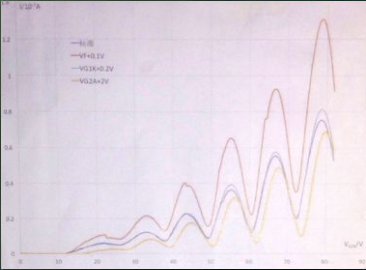
\includegraphics[height=10cm]{lab2151_1.png}
    \caption{四条曲线对比图(仅供参考,实际图片请根据实验数据自行绘制)}
	\end{figure}

\subsection*{5.示波器自动测量}

\begin{figure}[H]
	\centering
		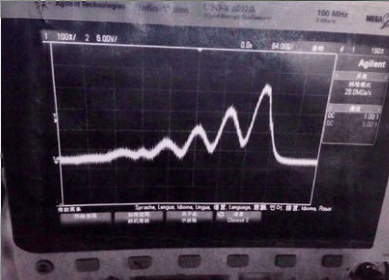
\includegraphics[height=10cm]{lab2151_2.png}
	\end{figure}



\end{document}